\section{Diseño de manipuladores robóticos}
% Robótica
Un manipulador robótico se define como una cadena cinemática abierta que puede programarse para realizar una amplia variedad de aplicaciones. La ingeniería mecánica proporciona un conjunto de metodologías para el estudio de máquinas en situaciones estáticas y dinámicas. Las ramas de la mecánica que permiten definir y estudiar el movimiento para el diseño de manipuladores robóticos, y de máquinas en general, son la \textbf{cinemática} y la \textbf{cinética}. De aquí en adelante, cinética y dinámica se utlizarán como sinónimos para seguir con la nomenclatura utilizada por los autores citados~\cite{craig}.

La \textbf{cinemática} trata el estudio del movimiento sin considerar las fuerzas que lo ocasionan. Se estudian la posición, la velocidad, la aceleración y todas las derivadas de mayor orden de la posición (respecto al tiempo o a cualquier otra variable). La \textbf{dinámica}, por otro lado, se encarga del estudio de las fuerzas sobre sistemas en movimiento. Permite definir los esfuerzos a los que estarán sometidos los elementos del sistema, como función de la aceleración y las fuerzas inerciales~\cite{norton}~\cite{craig}.

Los manipuladores se pueden considerar un tipo especial de \textbf{mecanismo}. Estos se definen, según Norton~\cite{norton}, como los dispositivos que transforman el movimiento en un patrón deseable y donde al menos uno de sus eslabones se ha \enquote{aterrizado} o fijado al sistema de referencia. Por lo general, desarrollan fuerzas muy bajas y transmiten poca potencia, a diferencia de las \textbf{máquinas} que están diseñadas para transmitir fuerzas significativas.

Para hablar de manipuladores robóticos, es necesario definir el concepto de cadena cinemática. Una \textbf{cadena cinemática} es un conjunto de eslabones, conectados por pares cinemáticos o juntas, que producen movimientos relativos sincronizados con un propósito determinado. Estas juntas generalmente se instrumentan con sensores de posición, que permiten conocer esta posición relativa de los eslabones adyacentes.~\cite{craig}

Un \textbf{eslabón} es un cuerpo rígido con al menos dos nodos o puntos de conexión. Se clasifican en binarios, ternarios y cuaternarios, dependiendo del número de nodos que posean. Una \textbf{junta o par cinemático} es la unión de dos o más eslabones en sus nodos, permitiendo movimiento relativo. Las juntas se pueden clasificar por sus grados de libertad (GDL) y las más comunes son las juntas completas (1 GDL) y las semijuntas (2 GDL), aunque también las hay de grados superiores.~\cite{norton}

%% Opcionalemente incluir la clasificación de cadenas cinemáticas

El número de grados de libertad globales de un manipulador es el número de variables de posición \textbf{independientes} que deben especificarse para conocer la posición de todos los eslabones de la cadena cinemática. Dicho de otra forma, es el número de entradas que se deben proporcionar para generar una salida predecible. Para determinarlo se debe de considerar el número de eslabones, el número de juntas y las interacciones entre ellos. La \textbf{condición de Gruebler} considera estos factores resumidos en la ecuación \ref{ec:kutzbach}.

\begin{equation}
\label{ec:kutzbach}
    M = 3(L-1)-2J_1-J_2
\end{equation}

donde:
\begin{description}
    \item[$M$] es el número de grados de libertad del mecanismo.
    \item[$L$] es el número total de eslabones, incluido el eslabón fijo.
    \item[$J_1$] es el número de pares cinemáticos de un grado de libertad.
    \item[$J_2$] es el número de pares cinemáticos de dos grados de libertad.
\end{description}
% Mecanismos

% Tipos de mecanismos

% Síntesis

% Análisis


\section{Variables de interés e instrumentación}


\section{Control de manipuladores robóticos}

La teoría de control proporciona herramientas para diseñar y evaluar algortimos para realizar los movimientos deseados o las aplicaciones de fuerza.

\section{\emph{Robot Operating System}}

El \emph{Robot Operating System (ROS)} es una plataforma (\emph{framework}) de código abierto orientada al desarrollo de sistemas en robótica. Su arquitectura facilita la comunicación y sincronización de los diferentes procesos encargados de las diferentes tareas que se deben realizar para el funcionamiento del sistema~\cite{ros_docs}.

Uno de los conceptos fundamentales de ROS es el \textbf{nodo}. Un nodo es un proceso que ejecuta una función específica dentro del sistema. Los nodos pueden comunicarse entre sí mediante diferentes mecanismos, permitiendo construir sistemas distribuidos en los que diferentes componentes pueden ejecutarse en distintas arquitecturas de hardware y con distintos sistemas operativos~\cite{ros_nodos}.

Las primeras distribuciones de ROS ya no cuentan con soporte actualmente. Su evolución es ROS 2 y fue diseñado para mejorar aspectos relacionados con tiempo real, seguridad, escalabilidad y aplicaciones comerciales e industriales. Una de sus principales diferencias es el uso del \emph{Data Distribution Service (DDS)} como infraestructura de comunicación. Esto permitió eliminar el proceso raíz, \emph{master}, encargado de la sincronización de los procesos.

ROS 2 proporciona principalmente tres mecanismos de comunicación~\cite{ros_interfaces}:

\begin{enumerate}
	\item \textbf{Tópicos:} Utilizan un modelo de publicador/suscriptor para la transmisión de datos de manera asíncrona. Son utilizados para sensores, estados del robot o comandos.
	\item \textbf{Servicios:} Utilizan un modelo de solicitud/respuesta y son apropiados para operaciones relativamente rápidas y discretas.
	\item \textbf{Acciones:} Permiten ejecutar tareas de mayor duración, proporcionando retroalimentación, un resultado final y la posibilidad de cancelar la operación.
\end{enumerate}

\section{Robot \emph{Justina}}

El Laboratorio de Bio-Robótica de la UNAM, fundado en 1997, se centra principalmente en la investigación de campos como visión artificial, reconocimiento de voz, planeación de tareas complejas, navegación y manipulación. Tiene la misión de promover el desarrollo de la ingeniería y la robótica en México. Con esta motivación, emprendió en 2005 la construcción de robots móviles destinados a ayudar a las personas en sus actividades cotidianas, en entornos domésticos, académicos, laborales y clínicos. Como resultado de esta labor, se construyó el robot de servicio de propósito general \emph{Justina}~\cite{justina_uv}.

\emph{Justina}, ver fig.~\ref{fig:justina}, desarrollada en su totalidad en el Laboratorio de Bio-Robótica, tiene el propósito de mejorar la calidad de vida de las personas. Su diseño se centra en facilitar la interacción con los humanos y con el ambiente. Todos los avances y mejoras que se incorporan son presentados anualmente en la categoría \emph{@HOME} de la RoboCup.

Actualmente, \emph{Justina} cuenta con una cámara RGBD, un micrófono direccional, un torso telescópico, un sensor LiDAR, dos brazos manipuladores con siete grados de libertad cada uno y una base móvil FESTO \emph{Robotino 4}. Por otro lado, el \emph{software} para controlar a Justina está organizado de manera modular, según el esquema del VirBot, ver fig.~\ref{fig:virbot}.

\begin{figure}[htbp]
    \centering
    \begin{subfigure}{0.5\textwidth}
        \centering
        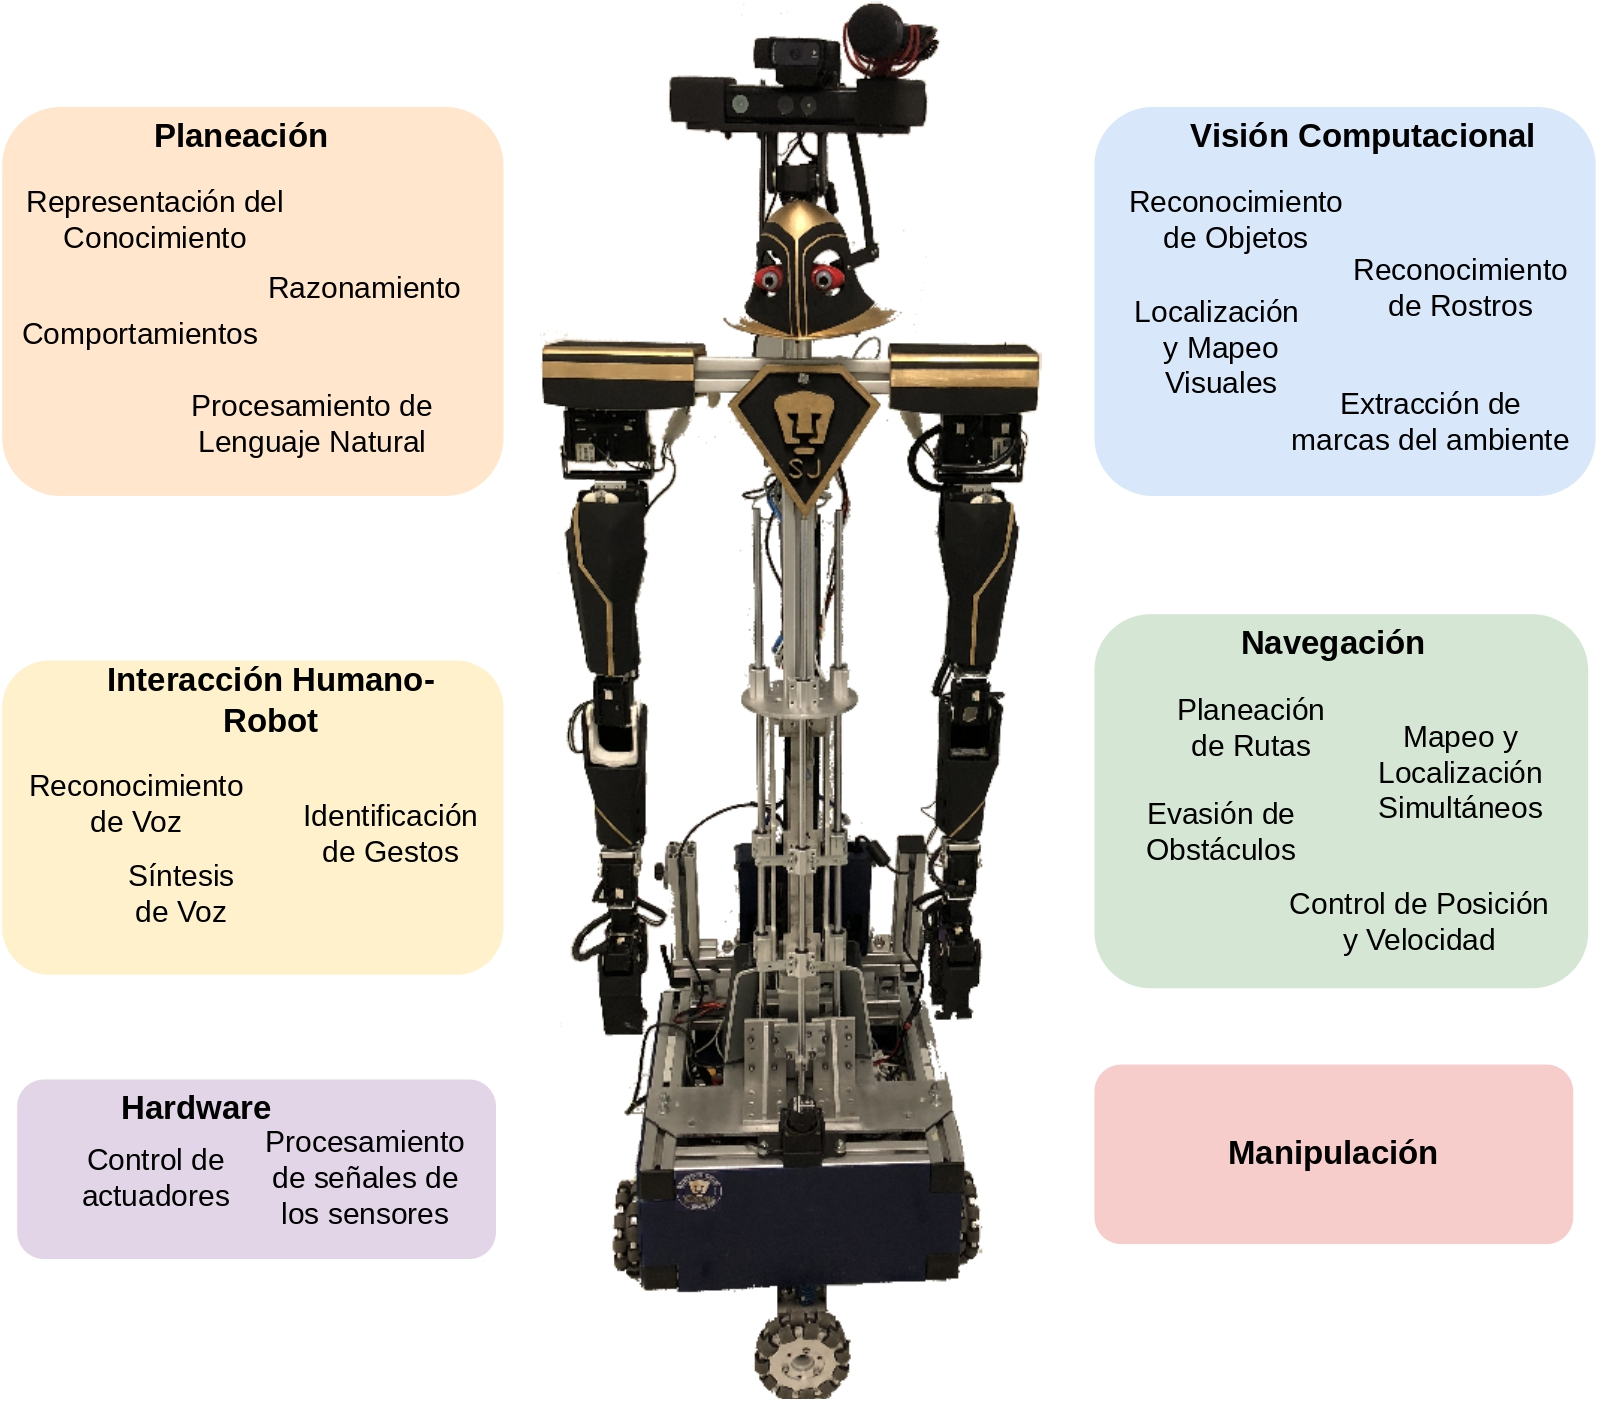
\includegraphics[width=\textwidth]{img/antecedentes/justina_subsystems.jpg}
        \caption{Justina}
        \label{fig:justina}
    \end{subfigure}
    \hfill
    \begin{subfigure}{0.42\textwidth}
        \centering
        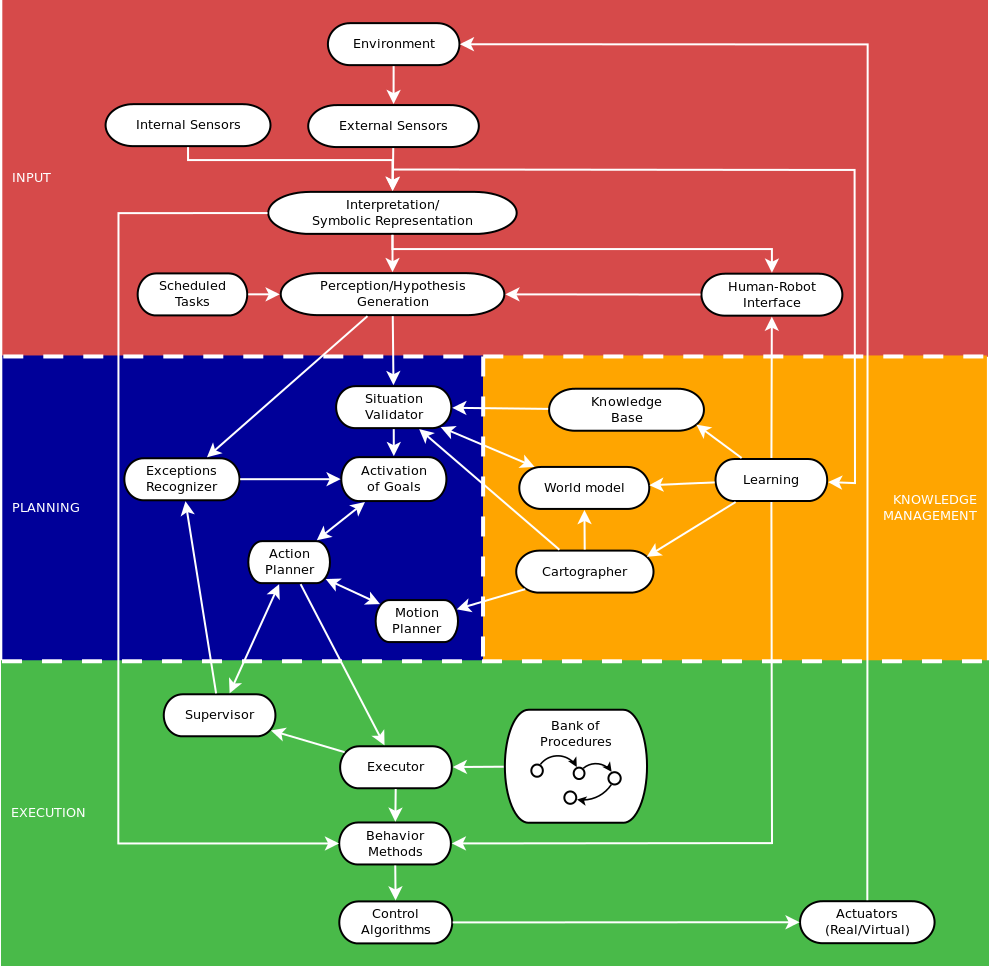
\includegraphics[width=\textwidth]{img/antecedentes/ViRBot_2.0.png}
        \caption{VirBot}
        \label{fig:virbot}
    \end{subfigure}
    \caption{Hardware y software de Justina}
\end{figure}

\section {Diseño centrado en el usuario}

Históricamente, el conocimiento práctico y la experiencia acumulada constituyeron la base del diseño. Como señalan Pahl y Beitz, a partir de la segunda mitad del siglo XX, la importancia económica del desarrollo eficiente y oportuno de productos motivó la creación de procedimientos sistemáticos y flexibles que permitieran planificar, optimizar, verificar y enseñar el proceso de diseño. Tal evolución propició la formalización de metodologías para analizar y descomponer problemas, generar soluciones óptimas y evaluar alternativas bajo criterios técnicos y económicos~\cite{Pahl-Beitz}. Estas metodologías, sin embargo, partían de especificaciones y requisitos que no consideraban a quienes usarían los productos.

El diseño centrado en el usuario (DCU) surgió en el laboratorio de Donald A. Norman en la Universidad de California San Diego como una filosofía que involucra al usuario en todas las fases del desarrollo de un producto, desde su conceptualización hasta su evaluación~\cite{Garreta-Mor}. Norman propuso en \textit{The Design of Everyday Things} un enfoque que parte de la comprensión profunda de las personas y de las necesidades que el diseño pretende satisfacer~\cite{Norman}. Este enfoque no es subjetivo, pues se fundamenta en disciplinas científicas como la ergonomía, la psicología y la antropología, y requiere que las decisiones de diseño estén respaldadas por datos obtenidos directamente de los usuarios~\cite{Lowdermilk}.

En aplicaciones domésticas de robótica de servicio, el DCU resulta especialmente pertinente. Robots como Justina demuestran capacidades de navegación, manipulación, visión e interacción humano-robot que les permiten operar en ambientes reales no estandarizados, adaptándose a los hogares y a sus habitantes~\cite{Rulebook@HOME}. Identificar sistemáticamente las necesidades de quienes conviven con estos sistemas es, por lo tanto, una condición necesaria para orientar el desarrollo de soluciones robóticas apropiadas.
